\documentclass[10pt,french]{book}
\input preambule_2013

\newcounter{exoc}
\newenvironment{exoc}[1]{%
  \refstepcounter{exoc}\textbf{Exercice \theexoc} :\hfill {\textbf{#1}}\par
  \medskip}%
{\medskip}

\begin{document}

%--------------------------------------------------
%       SUJET A
%--------------------------------------------------

\pieddepage{}{A}{}

\begin{center}
\begin{tabularx}{\textwidth}{|>\centering m{2.5cm}|>\centering X|>{\centering\arraybackslash} m{2.5cm}|}
	\hline
		1\iere \bsc{e.e.a.c.} & Mardi 15 octobre \np{2013} & \textbf{\'Etudes de fonctions} \\
	\hline
		\multicolumn{3}{|c|}{\bsc{Contrôle de mathématiques}} \\
	\hline
        \multicolumn{1}{|r}{\bsc{Nom}:} & \multicolumn{2}{l|}{} \\
		\multicolumn{1}{|r}{Prénom:} & \multicolumn{2}{l|}{} \\
	\hline
        \multicolumn{3}{|l|}{\bfseries Note et observations :} \\[1cm]
    \hline
\end{tabularx}\bigskip

{\itshape
La qualité et la précision de la rédaction seront prises en compte dans l'appréciation des copies.\par
Le barème est indicatif.}
\end{center}

\begin{exoc}{5 points}
    \begin{enumerate}
        \item Dessiner le tableau de variations de la fonction $x \mapsto \abs x$ pour $x \in \intervalleff{-5}{5}$.
        \item Résoudre dans $\R$ les équations suivantes : $\abs x = 3 \qq \abs x = \dfrac 14 \qq \abs x = -3$.
        \item Résoudre dans $\R$ les inéquations suivantes : $\abs x \leqslant 4 \qq \abs x > 5 \qq \abs x < -2$.
    \end{enumerate}\[*\]
\end{exoc}

\begin{exoc}{3 points}
\begin{minipage}{0.45\linewidth}
    Dans le repère $\left(O \pv \vect\imath, \vect\jmath\right)$ ci-contre, $\calig C_h$ représente la fonction valeur absolue. Les fonctions $f$ et $g$ sont respectivement représentées par $\calig C_f$ et $\calig C_g$.\par\medskip
    Donner l'expression de $f(x)$, $g(x)$ et $h(x)$ en fonction de $x$.
\end{minipage}\hfill\begin{minipage}{0.45\linewidth}
\begin{center}
    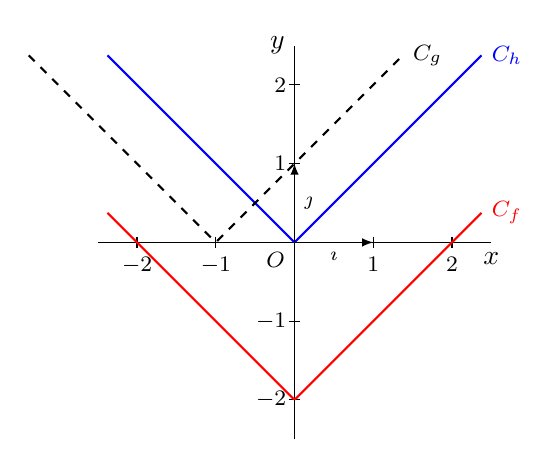
\begin{tikzpicture}[>=latex,x=0.5cm,y=0.5cm]
        \draw (-5,0) -- (5,0) node[below] {$x$} ;
        \foreach \x in {-2, -1,1,2} \draw[xshift=\x cm] (0pt,2pt) -- (0pt,-2pt) node[below] {\footnotesize$\x$};
        \draw (0,-5) -- (0,5) node[left] {$y$} ;
        \foreach \y in {-1,-2,1,2} \draw[yshift=\y cm] (-2pt,0pt) -- (2pt,0pt) node[left=1.5pt] {\footnotesize$\y$};
        \draw (0,0) node[below left] {\footnotesize $O$};
        \draw[blue,thick,domain=-4.75:4.75,samples=200]plot(\x,{abs(\x)}) node[right]{\footnotesize$\calig C_h$};
        \draw[red,thick,domain=-4.75:4.75,samples=200]plot(\x,{abs(\x) - 4}) node[right]{\footnotesize$\calig C_f$};
        \draw[thick,domain=-6.75:2.75,samples=200,dashed]plot(\x,{abs(\x + 2)}) node[right]{\footnotesize$\calig C_g$};
        \draw[->] (0,0) -- (2,0) node[midway,below] {\scriptsize$\vect\imath$};
        \draw[->] (0,0) -- (0,2) node[midway,right] {\scriptsize$\vect\jmath$};
    \end{tikzpicture}
\end{center}
\end{minipage}\[*\]
\end{exoc}

\begin{exoc}{2 points}
\begin{minipage}{0.45\linewidth}
    Dans le repère $\left(O \pv \vect\imath, \vect\jmath\right)$ ci-contre, $\calig C_f$ est la courbe représentative d'une fonction $f$ sur l'intervalle $[-2 \pv 2]$.\par\medskip
    Sur ce repère, représenter \textbf{soigneusement} la fonction $x \mapsto \abs{f(x)}$.
\end{minipage}\hfill\begin{minipage}{0.45\linewidth}
\begin{center}
    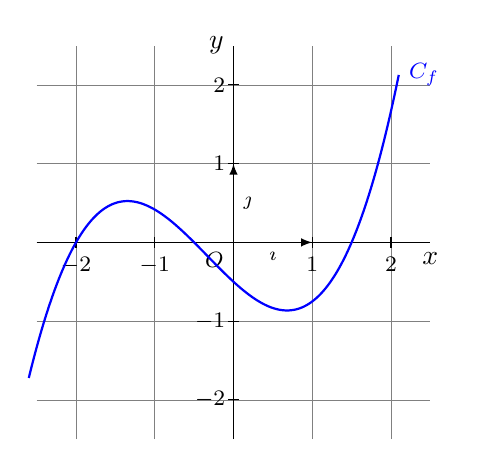
\begin{tikzpicture}[>=latex,x=0.5cm,y=0.5cm]
        \draw[help lines] (-5,-5) grid (5,5);
        \draw (-5,0) -- (5,0) node[below] {$x$} ;
        \foreach \x in {-2, -1,1,2} \draw[xshift=\x cm] (0pt,2pt) -- (0pt,-2pt) node[below] {\footnotesize$\x$};
        \draw (0,-5) -- (0,5) node[left] {$y$} ;
        \foreach \y in {-1,-2,1,2} \draw[yshift=\y cm] (-2pt,0pt) -- (2pt,0pt) node[left=1.5pt] {\footnotesize$\y$};
        \draw (0,0) node[below left] {\footnotesize $O$};
        \draw[blue,thick,domain=-5.2:4.2,samples=200]plot(\x,{(\x + 4)*(\x + 1)*(\x - 3)/12}) node[right]{\footnotesize$\calig C_f$};
        \draw[->] (0,0) -- (2,0) node[midway,below] {\scriptsize$\vect\imath$};
        \draw[->] (0,0) -- (0,2) node[midway,right] {\scriptsize$\vect\jmath$};
    \end{tikzpicture}
\end{center}
\end{minipage}\[*\]
\end{exoc}

\begin{exoc}{10 points}
Soient $a$, $b$ et $c$ les trois fonctions définies sur $\R$ par :
    \[a(x) = x^2 \qq b(x) = x^2 - 8x + 16 \qetq c(x) = (x - 3)(x + 3) + 5\]
On appelle $\calig C_a$, $\calig C_b$ et $\calig C_c$ leur représentation graphique respective.

\begin{enumerate}
    \item Factoriser l'expression $b(x)$ et prouver que $b(x) = a(x - 4)$.
    \item Développer et réduire l'expression $c(x)$ et prouver que $c(x) = a(x) - 4$.
    \item Par quelle transformation géométrique obtient-on :
        \begin{enumerate}
            \item $\calig C_b$ par rapport $\calig C_a$ ?
            \item $\calig C_c$ par rapport $\calig C_a$ ?
        \end{enumerate}
    \item Dans le repère ci-dessous, tracer \textbf{soigneusement} les représentations graphiques des fonctions $a$, $b$, $c$ et $\abs c$. \textbf{Utiliser des couleurs différentes.}
\end{enumerate}\[*\]
\end{exoc}

\begin{center}
    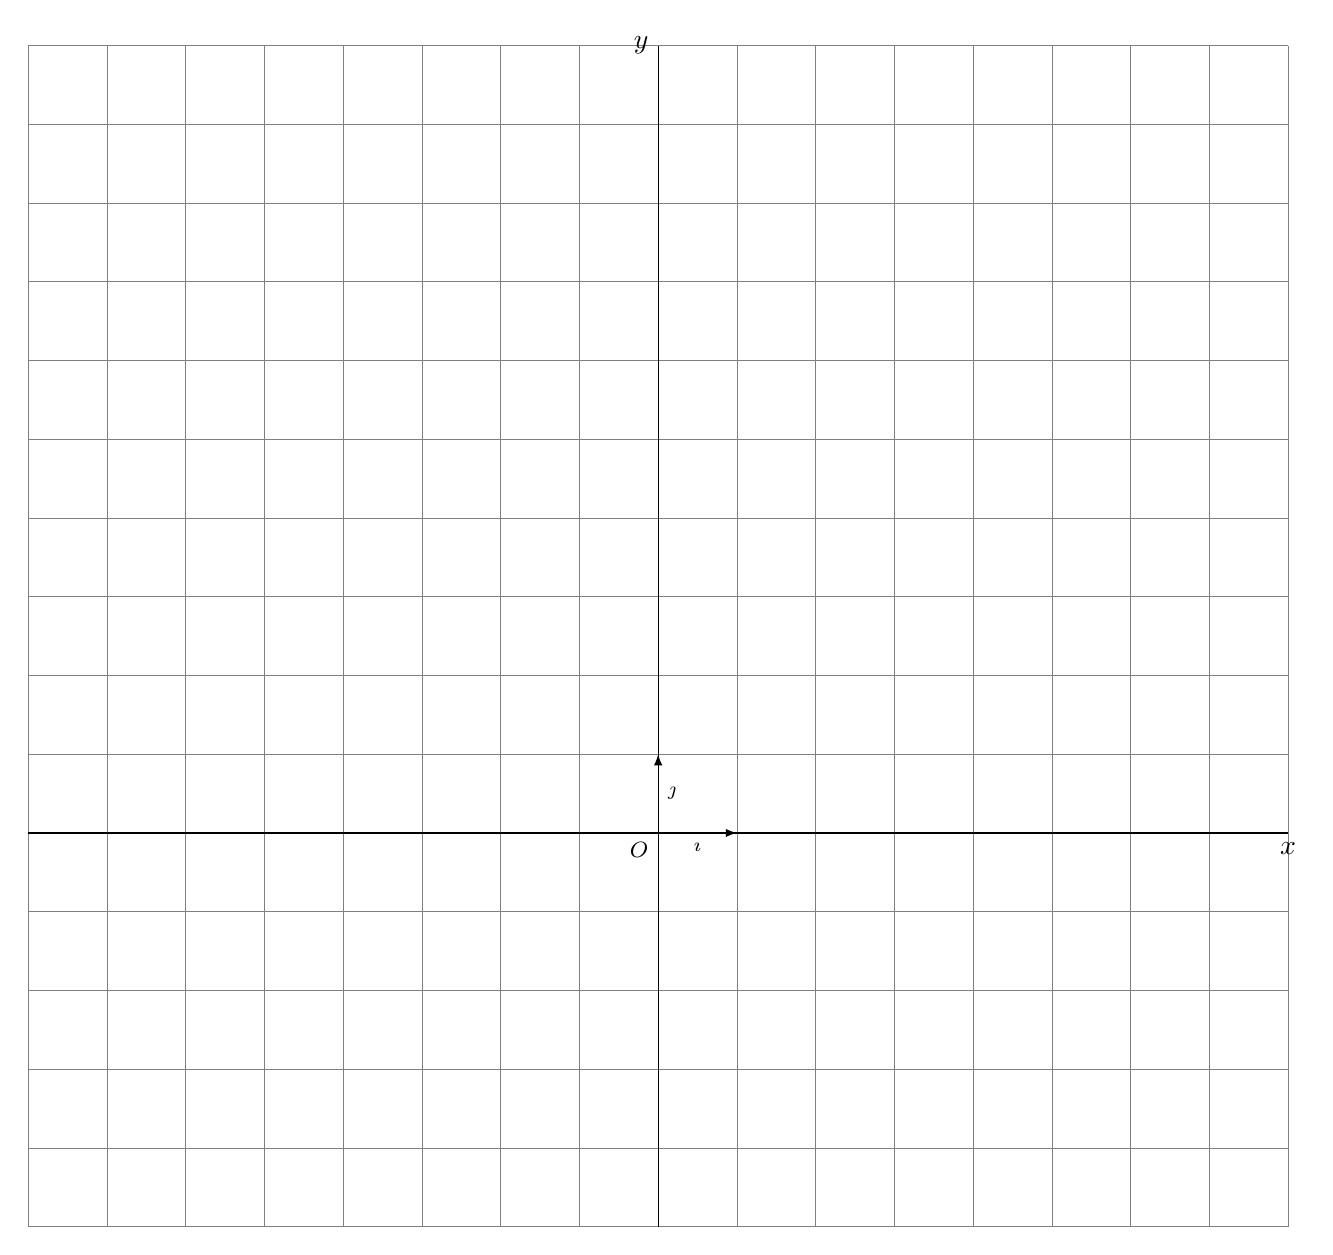
\begin{tikzpicture}[>=latex]
        \draw[help lines] (-8,-5) grid (8,10);
        \draw (-8,0) -- (8,0) node[below] {$x$} ;
        \draw (0,-5) -- (0,10) node[left] {$y$} ;
        \draw (0,0) node[below left] {\footnotesize $O$};
        \draw[->] (0,0) -- (1,0) node[midway,below] {\scriptsize$\vect\imath$};
        \draw[->] (0,0) -- (0,1) node[midway,right] {\scriptsize$\vect\jmath$};
    \end{tikzpicture}
\end{center}

\clearpage\setcounter{exoc}{0}

%--------------------------------------------------
%       SUJET B
%--------------------------------------------------

\pieddepage{}{B}{}

\begin{center}
\begin{tabularx}{\textwidth}{|>\centering m{2.5cm}|>\centering X|>{\centering\arraybackslash} m{2.5cm}|}
	\hline
		1\iere \bsc{e.e.a.c.} & Mardi 15 octobre \np{2013} & \textbf{\'Etudes de fonctions} \\
	\hline
		\multicolumn{3}{|c|}{\bsc{Contrôle de mathématiques}} \\
	\hline
        \multicolumn{1}{|r}{\bsc{Nom}:} & \multicolumn{2}{l|}{} \\
		\multicolumn{1}{|r}{Prénom:} & \multicolumn{2}{l|}{} \\
	\hline
        \multicolumn{3}{|l|}{\bfseries Note et observations :} \\[1cm]
    \hline
\end{tabularx}\bigskip

{\itshape
La qualité et la précision de la rédaction seront prises en compte dans l'appréciation des copies.\par
Le barème est indicatif.}
\end{center}

\begin{exoc}{5 points}
    \begin{enumerate}
        \item Dessiner le tableau de variations de la fonction $x \mapsto \abs x$ pour $x \in \intervalleff{-6}{6}$.
        \item Résoudre dans $\R$ les équations suivantes : $\abs x = 2 \qq \abs x = \dfrac 13 \qq \abs x = -1$.
        \item Résoudre dans $\R$ les inéquations suivantes : $\abs x \leqslant 3 \qq \abs x \geqslant 4 \qq \abs x > -2$.
    \end{enumerate}\[*\]
\end{exoc}

\begin{exoc}{3 points}
\begin{minipage}{0.45\linewidth}
    Dans le repère $\left(O \pv \vect\imath, \vect\jmath\right)$ ci-contre, $\calig C_h$ représente la fonction valeur absolue. Les fonctions $f$ et $g$ sont respectivement représentées par $\calig C_f$ et $\calig C_g$.\par\medskip
    Donner l'expression de $f(x)$, $g(x)$ et $h(x)$ en fonction de $x$.
\end{minipage}\hfill\begin{minipage}{0.45\linewidth}
\begin{center}
    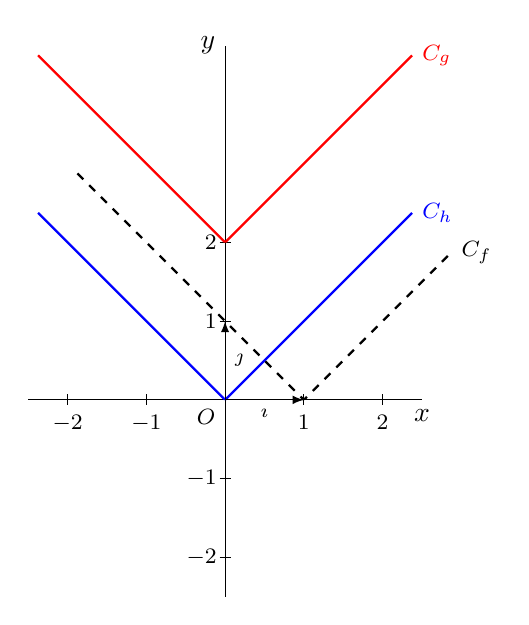
\begin{tikzpicture}[>=latex,x=0.5cm,y=0.5cm]
        \draw (-5,0) -- (5,0) node[below] {$x$} ;
        \foreach \x in {-2, -1,1,2} \draw[xshift=\x cm] (0pt,2pt) -- (0pt,-2pt) node[below] {\footnotesize$\x$};
        \draw (0,-5) -- (0,9) node[left] {$y$} ;
        \foreach \y in {-1,-2,1,2} \draw[yshift=\y cm] (-2pt,0pt) -- (2pt,0pt) node[left=1.5pt] {\footnotesize$\y$};
        \draw (0,0) node[below left] {\footnotesize $O$};
        \draw[blue,thick,domain=-4.75:4.75,samples=200]plot(\x,{abs(\x)}) node[right]{\footnotesize$\calig C_h$};
        \draw[red,thick,domain=-4.75:4.75,samples=200]plot(\x,{abs(\x) + 4}) node[right]{\footnotesize$\calig C_g$};
        \draw[thick,domain=-3.75:5.75,samples=200,dashed]plot(\x,{abs(\x - 2)}) node[right]{\footnotesize$\calig C_f$};
        \draw[->] (0,0) -- (2,0) node[midway,below] {\scriptsize$\vect\imath$};
        \draw[->] (0,0) -- (0,2) node[midway,right] {\scriptsize$\vect\jmath$};
    \end{tikzpicture}
\end{center}
\end{minipage}\[*\]
\end{exoc}

\begin{exoc}{2 points}
\begin{minipage}{0.45\linewidth}
    Dans le repère $\left(O \pv \vect\imath, \vect\jmath\right)$ ci-contre, $\calig C_f$ est la courbe représentative d'une fonction $f$ sur l'intervalle $[-2 \pv 2]$.\par\medskip
    Sur ce repère, représenter \textbf{soigneusement} la fonction $x \mapsto \abs{f(x)}$.
\end{minipage}\hfill\begin{minipage}{0.45\linewidth}
\begin{center}
    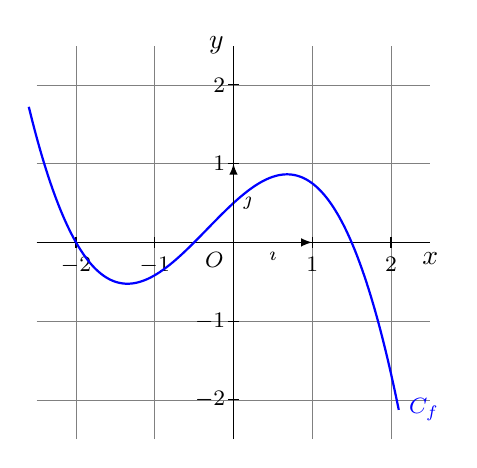
\begin{tikzpicture}[>=latex,x=0.5cm,y=0.5cm]
        \draw[help lines] (-5,-5) grid (5,5);
        \draw (-5,0) -- (5,0) node[below] {$x$} ;
        \foreach \x in {-2, -1,1,2} \draw[xshift=\x cm] (0pt,2pt) -- (0pt,-2pt) node[below] {\footnotesize$\x$};
        \draw (0,-5) -- (0,5) node[left] {$y$} ;
        \foreach \y in {-1,-2,1,2} \draw[yshift=\y cm] (-2pt,0pt) -- (2pt,0pt) node[left=1.5pt] {\footnotesize$\y$};
        \draw (0,0) node[below left] {\footnotesize $O$};
        \draw[blue,thick,domain=-5.2:4.2,samples=200]plot(\x,{-(\x + 4)*(\x + 1)*(\x - 3)/12}) node[right]{\footnotesize$\calig C_f$};
        \draw[->] (0,0) -- (2,0) node[midway,below] {\scriptsize$\vect\imath$};
        \draw[->] (0,0) -- (0,2) node[midway,right] {\scriptsize$\vect\jmath$};
    \end{tikzpicture}
\end{center}
\end{minipage}\[*\]
\end{exoc}

\begin{exoc}{10 points}
Soient $a$, $b$ et $c$ les trois fonctions définies sur $\R$ par :
    \[a(x) = x^2 - 10x + 25 \qq b(x) = x^2 \qetq c(x) = (x - 1)(x + 1) - 4\]
On appelle $\calig C_a$, $\calig C_b$ et $\calig C_c$ leur représentation graphique respective.

\begin{enumerate}
    \item Développer et réduire l'expression $c(x)$ et prouver que $c(x) = b(x) - 5$.
    \item Factoriser l'expression $a(x)$ et prouver que $a(x) = b(x - 5)$.
    \item Par quelle transformation géométrique obtient-on :
        \begin{enumerate}
            \item $\calig C_a$ par rapport $\calig C_b$ ?
            \item $\calig C_c$ par rapport $\calig C_b$ ?
        \end{enumerate}
    \item Dans le repère ci-dessous, tracer \textbf{soigneusement} les représentations graphiques des fonctions $a$, $b$, $c$ et $\abs c$. \textbf{Utiliser des couleurs différentes.}
\end{enumerate}\[*\]
\end{exoc}

\begin{center}
    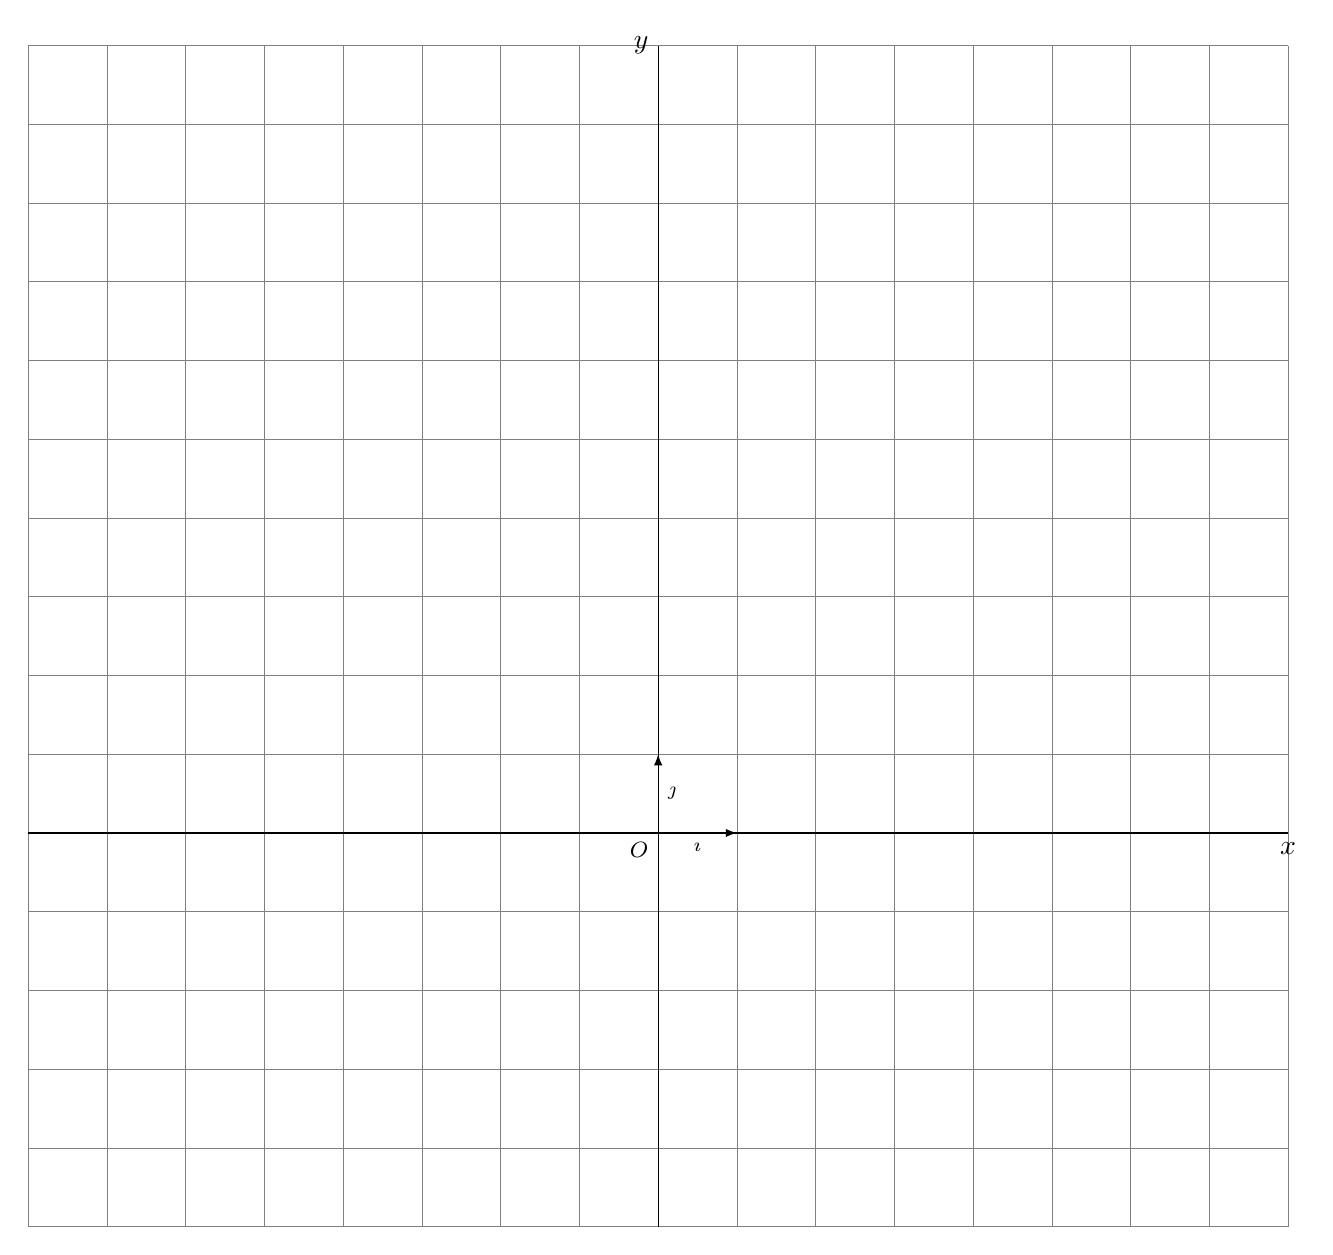
\begin{tikzpicture}[>=latex]
        \draw[help lines] (-8,-5) grid (8,10);
        \draw (-8,0) -- (8,0) node[below] {$x$} ;
        \draw (0,-5) -- (0,10) node[left] {$y$} ;
        \draw (0,0) node[below left] {\footnotesize $O$};
        \draw[->] (0,0) -- (1,0) node[midway,below] {\scriptsize$\vect\imath$};
        \draw[->] (0,0) -- (0,1) node[midway,right] {\scriptsize$\vect\jmath$};
    \end{tikzpicture}
\end{center}

\end{document} 